Kroz ovaj dio dokumenta su obrađeni \textbf{funckionalni zahtjevi} aplikacije "Reader", odnosno, oni zahtjevi koji specificiraju šta se očekuje od sistema (šta bi sistem trebao da radi), kako sistem reaguje na odgovarajuće ulaze i kako se sistem ponaša u određenim situacijama.\newline Funkcionalni zahtjevi ovog sistema se mogu podijeliti u sljedeće kategorije:
\begin{itemize}
    \item Korisnički računi
    \item Dodavanje pdf fajlova
    \item Čitanje pdf fajlova
    \item Izdvajanje dijelova dokumenta
\end{itemize}

\begin{center}
    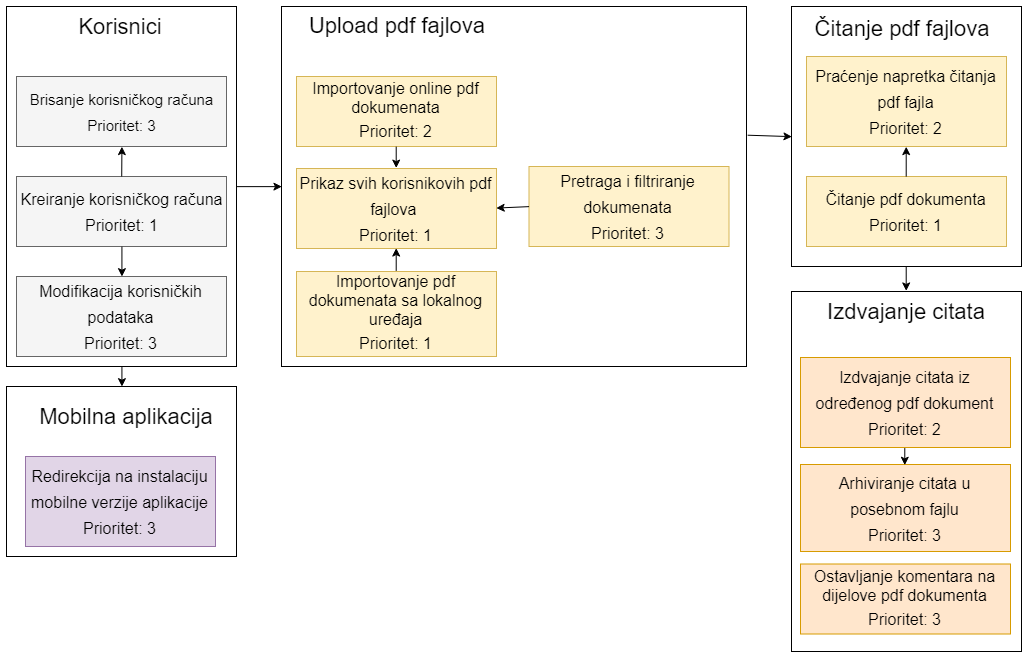
\includegraphics[scale=0.5]{images/dijagram.png}   
\end{center}

Kroz korisničke račune su obuhvaćene funkcionalnosti kreiranja, modifikovanja i brisanja kreiranog korisničkog računa. Dodavanje pdf fajlova uključuje importovanje pdf dokumenata sa lokalnog uređaja, importovanje online pdf dokumenata i prikaz svih korisnikovih dokumenata. Čitanje pdf fajlova podrazumijeva funkcionalnost otvaranja jednog pdf dokumenta i izdvajanje odgovarajućih dijelova tog dokumenta. Pored toga, vodi se računa i o tome da ponovno otvaranje nekog dokumenta prikazuje dokument počevši od pozicije na kojoj je završilo prethodno čitanje. Izdvajanje dijelova dokumenta nudi korisniku određene mogućnosti sa izdvojenim dijelovima. Te mogućnosti su dodavanje tih dijelova dokumenta u arhivu, proglašavanje tih dijelova dokumenta omiljenim citatom, označavanje tih dijelova dokumenta kao početne dijelove za naredno čitanje i slično. Detaljna specifikacija ovih funkcionalnosti je prikazana u nastavku dokumenta.


\subsection{Mobilna aplikacija}

\subsubsection{Redirekcija na instalaciju mobilne aplikacije\\}
\begin{tabular}{|
>{\columncolor[HTML]{FFCE93}}c |p{.70\textwidth}|} \hline
Funkcionalnost &Redirekcija na instalaciju mobilne aplikacije \\ \hline
Opis & \begin{tabular}[c]{@{}p{.70\textwidth}@{}} Ukoliko korisnik sistemu pristupa pomoću web browsera sa mobilnog uređaja, potrebno je obavijestiti korisnika o postojanju mobilne verzije i predložiti instalaciju iste radi boljeg korisničkog iskustva.\end{tabular} \\ \hline
Preduslovi  & \begin{tabular}[c]{@{}p{.70\textwidth}@{}}Korisnik pristupa aplikaciji putem mobitela.\end{tabular} \\ \hline
Ulaz    & \begin{tabular}[c]{@{}p{.70\textwidth}@{}}Potvrda da se želi instalirati mobilna aplikacij.a\end{tabular} \\ \hline
Uslovi validnosti  & \begin{tabular}[c]{@{}p{.70\textwidth}@{}}/\end{tabular} \\ \hline
Procesiranje   & \begin{tabular}[c]{@{}p{.70\textwidth}@{}}1. Korisnik otvara aplikaciju kroz web browser na mobilnom uređaju \\ 2. Sistem prikazuje obavještenje da postoji mobilna verzija aplikacije \\ 3. Sistem pita korisnika da li želi instalirati mobilnu verziju aplikacije (Odabir da ili ne) \\ 3. Ukoliko je odgovor da, sistem preusmjerava korisnika na Google Play store stranicu gdje se nalazi mobilna verzija\end{tabular} \\ \hline
Izlaz     & \begin{tabular}[c]{@{}p{.70\textwidth}@{}} Obavijest da postoji mobilna verzija aplikacije i odabir da li se želi instalirati ta verzija.\end{tabular} \\ \hline
Funkcionalni zahtjevi & \begin{tabular}[c]{@{}p{.70\textwidth}@{}}1. Sistem prepoznaje kada mu se pristupa sa mobilnog browsera \\ 2. Sistem vrši redirekciju na odgovarajuću adresu gdje se nalazi instalacija mobilne aplikacije (Google Play store)\end{tabular} \\ \hline
Prioritet realizacije & \begin{tabular}[c]{@{}p{.70\textwidth}@{}}Funkcionalnost koja ne igra značajnu ulogu u radu same web aplikacije ali je bitna za ugodnije korisničko iskustvo korisnika koji preferiraju mobilne uređaje. \\ Prioritet: III \end{tabular}\\ \hline
\end{tabular}


\subsection{Korisnički računi}


\subsubsection{Kreiranje korisničkog računa\\}

\begin{tabular}{|
>{\columncolor[HTML]{FFCE93}}c |p{.70\textwidth}|}
\hline
Opis & Nakon uspješnog unošenja potrebnih podataka i verifikacije, korisnik može da koristi usluge web aplikacije. \\ \hline
Preduslovi & Potrebno je da korisnik ima e-mail adresu pomoću koje kreira i verifikuje račun. \\ \hline
Ulaz & Osnovni lični podaci korisnika: ime, prezime i e-mail adresa. \\ \hline
Uslovi validnosti & Za uspješno kreiranje računa, potrebno je izvršiti verifikaciju preko prethdno unesenog e-maila. \\ \hline
Procesiranje & \begin{tabular}[c]{@{}p{.70\textwidth}@{}}1. Otvaranje stranice. \\ 2. Odabir opcije za registraciju. \\ 3. Prikaz polja za unos podataka apotrebnih za kreiranje računa. \\ 4. Unos osnovnih informacije: ime, prezime, te e-mail. \\ 5. Slanje e-maila na upisanu adresu u svrhu verifikacije korisnika.  \\ 6. Ukoliko je verifikacija uspješno izvršena, pojavljuje se poruka o uspješno kreiranom korisničkom računu. \end{tabular} \\ \hline
Izlaz & Obavijest o ishodu akcije, odnosno uspješnosti kreiranja korisničkog računa. \\ \hline
Funkcionalni zahtjevi & \begin{tabular}[c]{@{}p{.70\textwidth}@{}}1. Sistem omogućava kreiranje korisničkog računa.\\ 2. Sistem omogućava pristup svim uslugama aplikacije. \end{tabular} \\ \hline
Prioritet realizacije & Korisnički račun je neophodan da bi se pristupalo aplikaciji i njenim uslugama. Stoga je prioritet ove funkcionalnosti I. \\ \hline
\end{tabular}

\subsubsection{Brisanje korisničkog računa\\}

\begin{tabular}{|
>{\columncolor[HTML]{FFCE93}}c |p{.70\textwidth}|}
\hline
Funkcionalnost & Brisanje korisničkog računa \\ \hline
Opis & Funkcionalnost koja omogućava korisnicima da obrišu svoj korisnički račun. \\ \hline
Preduslovi & Korisnik je registrovan i prijavljen na sistem. \\ \hline
Ulaz & Zahtjev za brisanje korisničkog računa. \\ \hline
Uslovi validnosti & Potvrda lozinke. \\ \hline
Procesiranje &  \begin{tabular}[c]{@{}p{.70\textwidth}@{}}1. Korisnik se loguje.\\ 2. Korisnik zahtijeva brisanje korisničkog računa.\\ 3. Korisnik potvrđuje lozinku.\end{tabular}\\ \hline
Izlaz & Obavijest o uspješnom brisanju korisničkog računa \\ \hline
Funkcionalni zahtjevi & \begin{tabular}[c]{@{}p{.70\textwidth}@{}}1. Sistem pruža mogućnost brisanja korisnika iz baze podataka.\\ 2. Sistem briše sve korisničke bilješke i komentare.\\ 3. Sistem onemogućava ponovno logovanje korisnika.\end{tabular} \\ \hline
Prioritet realizacije & III. \\ \hline
\end{tabular} 



\subsubsection{Modifikacija korisničkih podataka\\}

\begin{tabular}{|
>{\columncolor[HTML]{FFCE93}}c |p{.70\textwidth}|}
\hline
Funkcionalnost & Modifikacija korisničkih podataka \\ \hline
Opis & Funkcionalnost koja omogućava korisnicima da vrše izmjene svog korisničkog računa. \\ \hline
Preduslovi & Korisnik je registrovan i prijavljen na sistem. \\ \hline
Ulaz & Izmijenjeni korisnički podaci. \\ \hline
Uslovi validnosti & \begin{tabular}[c]{@{}p{.70\textwidth}@{}}1. Potvrda lozinke.\\ 2. U slučaju promjene e-mail adrese, nova adresa mora biti ispravnog formata i mora se verifikovati.\end{tabular} \\ \hline
Procesiranje &  \begin{tabular}[c]{@{}p{.70\textwidth}@{}}1. Korisnik se loguje.\\ 2. Korisnik zahtijeva izmjenu korisničkih podataka.\\3. Korisnik unosi nove podatke. \\4. Korisnik potvrđuje lozinku.\end{tabular}\\ \hline
Izlaz & Obavijest o uspješno izvršenim modifikacijama. \\ \hline
Funkcionalni zahtjevi & \begin{tabular}[c]{@{}p{.70\textwidth}@{}}1. Sistem pruža mogućnost izmjene imena i prezimena.\\ 2. Sistem omogućava promjenu e-mail adrese pomoću koje je kreiran račun.\\ 3. Sistem onemogućava promjenu lozinke računa.\end{tabular} \\ \hline
Prioritet realizacije & III. \\ \hline
\end{tabular} 

\newpage
\subsection{Dodavanje pdf fajlova}

\subsubsection{Importovanje pdf dokumenata sa lokalnog uređaja\\}
\begin{tabular}{|
>{\columncolor[HTML]{FFCE93}}c |p{.70\textwidth}|} \hline
Funkcionalnost & Importovanje pdf dokumenata sa lokalnog uređaja  \\ \hline
Opis & \begin{tabular}[c]{@{}p{.70\textwidth}@{}}Potrebno je omogućiti da korisnik doda novi pdf dokument u svoju arhivu kako bi ga kasnije mogao čitati, označavati i izdvajati citate. Ovo podrazumijeva selektovanje željenog pdf dokumenta na lokalnom uređaju te njegovo pohranjivanje na sistem. (Upload)\end{tabular} \\ \hline
Preduslovi  & \begin{tabular}[c]{@{}p{.70\textwidth}@{}}1. Dokument postoji na lokalnom uređaju.\\ 2. Korisnik je registrovan i prijavljen na sistem.\end{tabular} \\ \hline
Ulaz    & \begin{tabular}[c]{@{}p{.70\textwidth}@{}}1. Ime dokumenta\\ 2. Pdf dokument\\ 3. Podaci o dokumentu (opcionalno)\end{tabular} \\ \hline
Uslovi validnosti  & \begin{tabular}[c]{@{}p{.70\textwidth}@{}}1. Dokument je validan i u odgovarajućem je formatu (.pdf)\\ 2. Korisnik importovanjem ne narušava autorska prava na dokument.\end{tabular} \\ \hline
Procesiranje   & \begin{tabular}[c]{@{}p{.70\textwidth}@{}}1. Odabir opcije za upload dokumenta.\\ 2. Odabir dokumenta.\\ 3. Unos imena dokumenta.\\ 4. Unos opisa dokumenta (po želji korisnika, u svrhu lakšeg pronalaženja dokumenta)\\ 5. Potvrda akcije.\end{tabular} \\ \hline
Izlaz     & \begin{tabular}[c]{@{}p{.70\textwidth}@{}} Obavijest o uspješnom prenosu dokumenta ili eventualnoj grešci te otvaranje dokumenta ukoliko je prenos obavljen uspješno.\end{tabular} \\ \hline
Funkcionalni zahtjevi & \begin{tabular}[c]{@{}p{.70\textwidth}@{}}1. Sistem omogućava online pohranu/skladištenje datoteka.\\ 2. Validacija na klijentu (forma za unos dokumenta).\\ 3. Validacija na serveru.\end{tabular} \\ \hline
Prioritet realizacije & \begin{tabular}[c]{@{}p{.70\textwidth}@{}}Ova funkcionalnost je među najbitnijim ako ne i najbitnija jer se na nju oslanjaju sve ključne funkcionalnosti sistema. \\ Priroritet: I \end{tabular}\\ \hline
\end{tabular}

\newpage
\subsubsection{Importovanje online pdf dokumenata\\}
\begin{tabular}{|
>{\columncolor[HTML]{FFCE93}}c |p{.70\textwidth}|} \hline
Funkcionalnost & Importovanje online pdf dokumenata \\ \hline
Opis & \begin{tabular}[c]{@{}p{.70\textwidth}@{}} Potrebno je korisniku omogućiti da u sistem importuje pdf dokumente koji nisu samo pohranjeni na njegovom lokalnom uređaju već se nalaze i na internetu. \end{tabular} \\ \hline
Preduslovi  & \begin{tabular}[c]{@{}p{.70\textwidth}@{}}1. Korisnik je registrovan i prijavljen na sistem \\ 2. Korisnik ima pristup online pdf dokumentu \\ 3. Dozvoljeno je preuzimanje pdf dokumenta sa date lokacije
\end{tabular} \\ \hline
Ulaz    & \begin{tabular}[c]{@{}p{.70\textwidth}@{}}1. Ime dokumenta \\ 2. Link na pdf dokument \\ 3. Podaci o dokumentu (opcionalno)\end{tabular} \\ \hline
Uslovi validnosti  & \begin{tabular}[c]{@{}p{.70\textwidth}@{}}1. Dokument je validan i u odgovarajućem je formatu (.pdf) \\ 2. Korisnik importovanjem ne narušava autorska prava na dokument \end{tabular} \\ \hline
Procesiranje   & \begin{tabular}[c]{@{}p{.70\textwidth}@{}}1. Odabir opcije za online import dokumenta \\ 2. Unos linka na dokument \\ 3. Unos imena dokumenta \\ 4. Unos dodatnog opisa dokumenta (po želji korisnika, u svrhu lakšeg prepoznavanja dokumenta) \\ 5. Potvrda akcije\end{tabular} \\ \hline
Izlaz & \begin{tabular}[c]{@{}p{.70\textwidth}@{}}Obavijest o uspješnom prenosu dokumenta ili eventualnoj grešci te otvaranje dokumenta ukoliko je prenos obavljen uspješno. \end{tabular} \\ \hline
Funkcionalni zahtjevi & \begin{tabular}[c]{@{}p{.70\textwidth}@{}}1. Sistem omogućava online pohranu/skladištenje datoteka \\ 2. Validacija na klijentu (forma za unos dokumenta) \\ 3. Validacija na serveru\end{tabular} \\ \hline
Prioritet realizacije & \begin{tabular}[c]{@{}p{.70\textwidth}@{}} Ova funkcionalnost iako nije neophodna za osnovno funkcionisanje sistema predstavlja jednu veoma važnu stavku po pitanju ugodnog korisničkog iskustva.\\  Prioritet: II. \end{tabular} \\ \hline
\end{tabular}

\newpage
\subsubsection{Prikaz svih korisnikovih pdf dokumenata\\}
\begin{tabular}{|
>{\columncolor[HTML]{FFCE93}}c |p{.70\textwidth}|} \hline
Funkcionalnost & Prikaz korisnikovih pdf dokumenata  \\ \hline
Opis & \begin{tabular}[c]{@{}p{.70\textwidth}@{}} Potrebno je omogućiti korisniku uvid u sve pdf dokumente koje je uploadovao na svoj korisnički račun. Korisnik može vidjeti nekolicinu dokumenata na svojoj početnoj stranici (dokumenti sa kojima je nedavno rađeno), a može i imati uvid u sve svoje dokumentom odlaskom na index stranicu (biblioteku). Na ovoj stranici moguće je prikazati i detaljnije informacije o nekom dokumentu.\end{tabular}  \\ \hline
Preduslovi  & \begin{tabular}[c]{@{}p{.70\textwidth}@{}}1. Korisnik je registrovan i prijavljen na sistem. \\ 2. Korisnik ima barem jedan pdf dokument u svojoj biblioteci.\end{tabular} \\ \hline
Ulaz    & \begin{tabular}[c]{@{}p{.70\textwidth}@{}}1. Broj prikazanih dokumenata po stranici (predefinisano) \\ 2. Broj stranice (Ukoliko je odabrani broj dokumenata po stranici manji od ukupnog broja dokumenata)
\end{tabular} \\ \hline
Uslovi validnosti  & \begin{tabular}[c]{@{}p{.70\textwidth}@{}}/\end{tabular} \\ \hline
Procesiranje   & \begin{tabular}[c]{@{}p{.70\textwidth}@{}}1. Prikaz nekolicine dokumenata na početnoj stranici. \\ 2. Klik na opciju “Index” u slučaju kad se želi uvid u sve dokumente.\end{tabular} \\ \hline
Izlaz & \begin{tabular}[c]{@{}p{.70\textwidth}@{}} Lista sa m prikazanih dokumenata (od ukupno m), uz opciju prikazivanja idućih/prethodnih m dokumenata ovisno o broju stranice i broju dokumenata po stranici.\end{tabular} \\ \hline
Funkcionalni zahtjevi & \begin{tabular}[c]{@{}p{.70\textwidth}@{}}1. Sistem podržava uvid u pohranjene pdf dokumente. \end{tabular} \\ \hline
Prioritet realizacije & \begin{tabular}[c]{@{}p{.70\textwidth}@{}} Funkcionalnost koja je veoma bitna s obzirom da pomoću nje korisnik ima uvid u listu svojih dokumenata. Također na ovu funkcionalnost se oslanja i funkcionalnost čitanja dokumenata s obzirom da ona predstavlja jedan način na koji se može pristupiti određenom dokumentu koji je uploadovan u prošlosti. \\ Prioritet: I. \end{tabular} \\ \hline
\end{tabular}

 \newpage
\subsubsection{Pretraga i filtriranje dokumenata\\}
\begin{tabular}{|
>{\columncolor[HTML]{FFCE93}}c |p{.70\textwidth}|} \hline
Funkcionalnost & Pretraga i filtriranje dokumenata \\ \hline
Opis & \begin{tabular}[c]{@{}p{.70\textwidth}@{}}Na ovoj stranici dostupni su filteri pomoću kojih je moguće prikazati određeni podskup korisnikovih dokumenata koji će se prikazati. Primjer filtera je polje za pretragu po imenu gdje korisnik unosi string, a rezultat pretraživanja se mijenja kako se mijenja i string.\end{tabular} \\ \hline
Preduslovi  & \begin{tabular}[c]{@{}p{.70\textwidth}@{}}1. Korisnik je registrovan i prijavljen na sistem. \\ 2. Korisnik ima barem jedan pdf dokument u svojoj biblioteci. \\ 3. Korisnik se nalazi na index stranici (Uvid u sve dokumente).\end{tabular} \\ \hline
Ulaz    & \begin{tabular}[c]{@{}p{.70\textwidth}@{}}1. String za pretragu po imenu \end{tabular} \\ \hline
Uslovi validnosti  & \begin{tabular}[c]{@{}p{.70\textwidth}@{}}1. String mora imati bar jedan znak da bi se prikazali dokumenti.
\end{tabular} \\ \hline
Procesiranje   & \begin{tabular}[c]{@{}p{.70\textwidth}@{}}1. Unos stringa za pretragu. \\ 2. Prikaz rezultata pretraživanja (dokumenata čiji naziv odgovara unesenom dijelu stringa u polje pretrage).\end{tabular} \\ \hline
Izlaz & \begin{tabular}[c]{@{}p{.70\textwidth}@{}}Lista dokumenata čiji naziv odgovara unesenom stringu (ili dijelu stringa) ili poruka da ne postoje dokumenti čiji naziv sadrži (trenutno uneseni) string.\end{tabular} \\ \hline
Funkcionalni zahtjevi & \begin{tabular}[c]{@{}p{.70\textwidth}@{}}1. Sistem omogućava pretraživanje dokumenata po imenu \\2. Pretraživanje je optimizovano\end{tabular} \\ \hline
Prioritet realizacije & \begin{tabular}[c]{@{}p{.70\textwidth}@{}}Ova funkcionalnost nije neophodna za funkcionisanje sistema i karakterizira se kao nice-to-have funkcionalnost. \\ Prioritet: III.\end{tabular}\\ \hline
\end{tabular}

\newpage
\subsection{Čitanje pdf fajlova\\}
\subsubsection{Čitanje pdf dokumenta\\}

\begin{tabular}{|
>{\columncolor[HTML]{FFCE93}}c |p{.70\textwidth}|}
\hline
\multicolumn{1}{|1|}{\cellcolor[HTML]{FFCE93}Funkcionalnost} & Čitanje pdf dokumenta \\ \hline
Opis & Funkcionalnost koja omogućava otvaranje (prethodno dodanih) pdf dokumenata i prolazak kroz sadržaj istog,uz mogućnosti selektovanja određenih dijelova dokumenata. \\ \hline
Preduslovi & Dokument koji se želi pročitati je već upload-ovan ili se nalazi na mobilnom uređaju. \\ \hline
Ulaz & Dokument koji korisnik želi da čita. \\ \hline
Uslovi validnosti & / \\ \hline
Procesiranje & Korisnik bira dokument koji želi da pročita (klikom na taj dokument), nakon čega se odabrani dokument prikazuje preko cijelog ekrana. Ukoliko korisnik selektuje određeni dio dokumenta, prikazuju mu se opcije da selektovani dio kopira, doda u neku arhivu, proglasi omiljenim citatom ili označi kao liniju od koje želi nastaviti čitanje pri narednom otvaranju dokumenta. U zavisnosti od toga šta korisnik izabere, provodi se odgovarajuća akcija. \\ \hline
Izlaz & Obavijest o uspješno izvršenim (odabranim) akcijama. \\ \hline
Funkcionalni zahtjevi & \begin{tabular}[c]{@{}p{.70\textwidth}@{}}1. Sistem pruža mogućnost otvaranja dokumenata.\\ 2. Sistem pruža mogućnost selektovanja određenih dijelova dokumenta koji se trenutno čita.\\ 3. Sistem pruža mogućnost kopiranja selektovanog dijela teksta.\\ 4. Sistem pruža mogućnost dodavanja izdvojenog dijela u arhivu.\\ 5. Sistem pruža mogućnost označavanja izdvojenog dijela kao omiljenog citata.\\ 6. Sistem pruža mogućnost označavanja dijela dokumenta od kojeg se želi započeti naredno čitanje tog dokumenta.\end{tabular} \\ \hline
Prioritet realizacije & Obzirom da je ova funkcionalnost neophodna za aplikaciju, njen prioritet realizacije je I. \\ \hline
\end{tabular}

\newpage
\subsubsection{Praćenje napretka čitanja pdf fajla\\}

\begin{tabular}{|
>{\columncolor[HTML]{FFCE93}}c |p{.70\textwidth}|}
\hline
Funkcionalnost & Praćenje napretka čitanja pdf dokumenta \\ \hline
Opis & Funkcionalnost koja omogućava korisnicima da svako naredno čitanje istog pdf dokumenta počnu tamo gdje je prethodno čitanje tog dokumenta završilo. \\ \hline
Preduslovi & Dokument je prethodno već čitan. \\ \hline
Ulaz & Dokument koji korisnik želi (ponovo) čitati. \\ \hline
Uslovi validnosti & Korisnik je prilikom prethodnog čitanja odabrao poziciju sa koje želi početi novo čitanje tog dokumenta. \\ \hline
Procesiranje & Korisnik otvara dokument koji je ranije čitan (klikom na taj dokument). Nakon toga, dokument se otvara preko cijelog ekrana, pri čemu je prva stranica koja se prikazuje ona na kojoj se nalazi tekst od kojeg korisnik želi nastaviti novo čitanje (a koji je označio priprethodnom čitanju). U otvorenom dokumentu su drugom bojom označeni svi citati koje je korisnik proglasio omiljenim u prethodnim čitanjima. Tokom čitanja dokumenata, korisnik ima sva prava kao i pri prvom otvaranju dokumenta. \\ \hline
Izlaz & Obavijest o uspješno izvršenim (odabranim) akcijama. \\ \hline
Funkcionalni zahtjevi & \begin{tabular}[c]{@{}p{.70\textwidth}@{}}1. Sistem pruža mogućnost ponovnog čitanja dokumenta, pri čemu čitanje počinje tamo gdje je prethodno završilo.\\ 2. Sistem prikazuje ranije označene citate drugom bojom.\\ 3. Sistem pruža sve mogućnosti navedene kroz opis prethodnog funkcionalnog zahtjeva.\end{tabular} \\ \hline
Prioritet realizacije & Obzirom da ova funkcionalnost predstavlja dodatak na prethodnu, prioritet njene realizacije je II. \\ \hline
\end{tabular}   

\subsection{Izdvajanje dijelova dokumenta}

\subsubsection{Izdvajanje citata iz određenog pdf dokumenta}
\begin{tabular}{|
>{\columncolor[HTML]{FFCE93}}c |l|}
\hline
Funkcionalnost        & Izdvajanje citata iz određenog pdf dokumenta                                                                                                                                                                                                            \\ \hline
Opis                  & \begin{tabular}[c]{@{}l@{}}Potrebno je omogućiti da korisnik izdvaja citate \\ iz pdf-dokumenta koji čita.\end{tabular}                                                                                                                                 \\ \hline
Preduslovi            & \begin{tabular}[c]{@{}l@{}}1. Korisnik je registrovan i prijavljen na sistem\\ 2. Dokument je otvoren za čitanje\\ 3. Korisnik je označio dio teksta koji želi spasiti\end{tabular}                                                                     \\ \hline
Ulaz                  & 1. Označen dio teksta koji se treba izdvojiti                                                                                                                                                                                                           \\ \hline
Uslovi validnosti     & \begin{tabular}[c]{@{}l@{}}1. Označen je odabrani citat u tekstu\\ 2. Korisnik mora odabrati opciju da li želi spasiti \\ citat u odvojeni dokument ili samo označiti \\ dokument\end{tabular}                                                          \\ \hline
Procesiranje          & \begin{tabular}[c]{@{}l@{}}1. Odabir pdf fajla za čitanje\\ 2. Otvaranje dokumenta za čitanje\\ 3. Selektovanje odabranog citata\\ 4. Odabir vizualnog načina za označavanje citata\\ 5. Odabir da li će se citat spašavati u zaseban fajl\end{tabular} \\ \hline
Izlaz                 & \begin{tabular}[c]{@{}l@{}}Obavijest o uspješno sačuvanom citatu. Vizualno \\ označavanje citata u tekstu. Spašavanje citata u \\ zaseban fajl u slučaju da je ta opcija odabrana.\end{tabular}                                                         \\ \hline
Funkcionalni zahtjevi & 1. Sistem omogućava online pohranu/skladištenje datoteka                                                                                                                                                                                                \\ \hline
Prioritet realizacije & \begin{tabular}[c]{@{}l@{}}Ova funkcionalnost olakšava korisniku izdvajanje citata. \\ S obzirom da je to dodatak funkcionalnosti čitanja pdf \\ dokumenta prioritet je II.\end{tabular}                                                                 \\ \hline
\end{tabular}

\subsubsection{Arhiviranje citata u posebnom fajlu}
\begin{tabular}{|
>{\columncolor[HTML]{FFCE93}}c |l|}
\hline
Funkcionalnost        & Arhiviranje citata u posebnom fajlu                                                                                                                                                                                                                             \\ \hline
Opis                  & \begin{tabular}[c]{@{}l@{}}Potrebno je omogućiti da korisnik arhivira citate \\ iz pdf-dokumenta koji čita u zaseban fajl.\end{tabular}                                                                                                                         \\ \hline
Preduslovi            & \begin{tabular}[c]{@{}l@{}}1. Korisnik je registrovan i prijavljen na sistem \\ 2. Dokument je otvoren za čitanje\\ 3. Korisnik je označio dio teksta koji želi arhivirati\end{tabular}                                                                         \\ \hline
Ulaz                  & \begin{tabular}[c]{@{}l@{}}1. Označen dio teksta koji se treba izdvojiti\\ 2. Odabrana opcija za arhiviranje citata u zaseban fajl\end{tabular}                                                                                                                 \\ \hline
Uslovi validnosti     & \begin{tabular}[c]{@{}l@{}}1. Označen je odabrani citat u tekstu\\ 2. Korisnik je odabrao opciju da želi spasiti citat u zaseban \\ fajl\end{tabular}                                                                                                           \\ \hline
Procesiranje          & \begin{tabular}[c]{@{}l@{}}Odabir pdf fajla za čitanje\\ Otvaranje dokumenta za čitanje\\ Selektovanje odabranog citata\\ Odabir vizualnog načina za označavanje citata\\ Odabir opcije za arhiviranje citata u zaseban fajl\\ Odabir naziva fajla\end{tabular} \\ \hline
Izlaz                 & \begin{tabular}[c]{@{}l@{}}Obavijest o uspješno sačuvanom citatu. Kreiranje novog \\ fajla sa odabranim imenom. Spašavanje citata u zaseban fajl.\end{tabular}                                                                                                  \\ \hline
Funkcionalni zahtjevi & 1. Sistem omogućava online pohranu/skladištenje datoteka                                                                                                                                                                                                        \\ \hline
Prioritet realizacije & \begin{tabular}[c]{@{}l@{}}Ova funkcionalnost je dodatak na funkcionalnost za \\ označavanje citata, s obzirom da prethodno trebaju \\ biti implementirani čitanje i označavanje citata, prioritet \\ realizacije je III.\end{tabular}                            \\ \hline
\end{tabular}

\subsubsection{Ostavljanje komentara na dijelove pdf dokumenta}
\begin{tabular}{|
>{\columncolor[HTML]{FFCE93}}c |l|}
\hline
Funkcionalnost        & Ostavljanje komentara na dijelove pdf dokumenta                                                                                                                                                                                                                           \\ \hline
Opis                  & \begin{tabular}[c]{@{}l@{}}Potrebno je omogućiti da korisnik piše i spašava \\ komentare na dijelove pdf dokumenta koji čita.\end{tabular}                                                                                                                                \\ \hline
Preduslovi            & \begin{tabular}[c]{@{}l@{}}1. Korisnik je registrovan i prijavljen na sistem \\ 2. Dokument je otvoren za čitanje\\ 3. Korisnik je označio dio teksta na koji želi dodati komentar\end{tabular}                                                                           \\ \hline
Ulaz                  & \begin{tabular}[c]{@{}l@{}}1. Označen dio fajla na koji se želi dodati komentar\\ 2. Odabrana opcija za dodavanje komentara\\ 3. Upisan tekst u polje za unos komentara\\ 4. Pritisnuto dugme za spašavanje komentara\end{tabular}                                        \\ \hline
Uslovi validnosti     & \begin{tabular}[c]{@{}l@{}}1. Označen je dio teksta na koji se treba dodati komentar\\ 2. Korisnik je odabrao opciju da želi dodati komentar\\ 3. Korisnik je unio komentar u polje za unos\\ 4. Korisnik je odabrao da želi spasiti napisani komentar\end{tabular}       \\ \hline
Procesiranje          & \begin{tabular}[c]{@{}l@{}}1. Odabir pdf fajla za čitanje\\ 2. Otvaranje dokumenta za čitanje\\ 3. Selektovanje odabranog dijela teksta\\ 4. Odabir opcije za dodavanje komentara\\ 5. Pisanje teksta za komentar\\ 6. Odabir opcije za spašavanje komentara\end{tabular} \\ \hline
Izlaz                 & \begin{tabular}[c]{@{}l@{}}Obavijest o uspješno sačuvanom komentaru. Vizualni \\ prikaz dijela na tekstu gdje se nalazi komentar.\end{tabular}                                                                                                                            \\ \hline
Funkcionalni zahtjevi & 1. Sistem omogućava online pohranu/skladištenje datoteka                                                                                                                                                                                                                  \\ \hline
Prioritet realizacije & \begin{tabular}[c]{@{}l@{}}Ova funkcionalnost je alternativa za spašavanje citata, ali \\ ima manji prioritet, te je zbog toga prioritet III.\end{tabular}                                                                                                                  \\ \hline
\end{tabular}